\section{Method of the characteristics}

\manuelComment{based on this video: https://www.youtube.com/watch?v=LpHqrlrU5pM}

The method of the characteristics is a powerful method to solve PDE. This method enable us to solve a wide range of problems including:
\begin{enumerate}
  \item Linear:
  \begin{equation}
  a(x, y) \frac{\partial u}{\partial x}
  + b(x, y) \frac{\partial u}{\partial y}
  + c(x, y) u
  = f(x, y)
  \end{equation}
  \item Semi-linear:
  \begin{equation}
  a(x, y) \frac{\partial u}{\partial x}
  + b(x, y) \frac{\partial u}{\partial y}
  + c(x, y) u
  = f(x, y, u)
  \end{equation}
  \item  Quasi-linear:
  \begin{equation}
  a(x, y) \frac{\partial u}{\partial x}
  + b(x, y) \frac{\partial u}{\partial y}
  = f(x, y, u)
  \end{equation}
\end{enumerate}

In this introduction  we will focus on semi-linear problems that also include
the linear ones. Let us consider a PDE of the form
\begin{equation}
  a(x, y) \frac{\partial u}{\partial x}
  + \b(x, y) \frac{\partial u}{\partial y}
  = f(x, y, u),
  \label{eq_semi_linear}
\end{equation}
which is a semi-linear PDE. Semi-linear equations include equations of the form
\begin{equation}
  a(x, y) \frac{\partial u}{\partial x}
  + \b(x, y) \frac{\partial u}{\partial y}
  + c(x, y) u
  = g(x, y),
\end{equation}
with $f(x, y, u) = g(x, y) - c(x, y) u$.

This PDE must have an initial condition associated with it. This initial
condition can be of the form
\begin{equation}
  u(x, 0) = u_0(x),
\end{equation}
or
\begin{equation}
  u(0, y) = u_1(x).
\end{equation}
The pair of a PDE like \eref[eq_semi_linear] and an initial condition is known
as a semi-linear Cauchy problem.

Any solution to these Cauchy problems can be represented by a surface $u \equiv
u(x, y)$ in a 3D space as schematically shown in \fref[fig_integral_surface]
\begin{figure}[h!]
	\centering 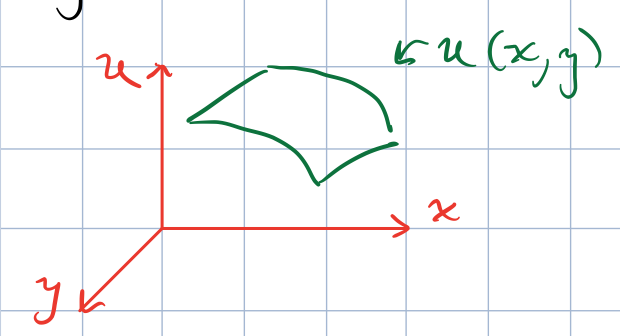
\includegraphics[scale=.75]{fig/fig1_method_characteristics.png}
	\caption{\captionStroke{Schematic integral surface.}}
	\label{fig_integral_surface}
\end{figure}

A surface $u = u(x, y)$ that solves a Cauchy problem is known as an integral
surface since integration is used to solve these problems. We can write down the
equation of this integral surface as
\begin{equation}
  F(x, y, u) \equiv u(x, y) - u = 0.
\end{equation}
Note that the first $u(x, y)$ is a function, while the second $u$ is a
variable. So for example if
\begin{equation}
  u(x, y) = x - y^2,
\end{equation}
then
\begin{equation}
  F(x, y, u) = x - y^2 - u.
\end{equation}

From vector calculus we know that any vector $\mathbf{n}$ normal to the surface $F = 0$ is given by the gradient
\begin{equation}
  \mathbf{n} = \nabla F =
  \frac{\partial u}{\partial x} \mathbf{i}
  + \frac{\partial u}{\partial y} \mathbf{j}
  - \mathbf{k}.
\end{equation}

\fref[fig_normal_vector] shows a schematic representation of this vector. The
vector is represented pointing downwards since $F = u(x, y) - u$.

\begin{figure}[h!]
	\centering 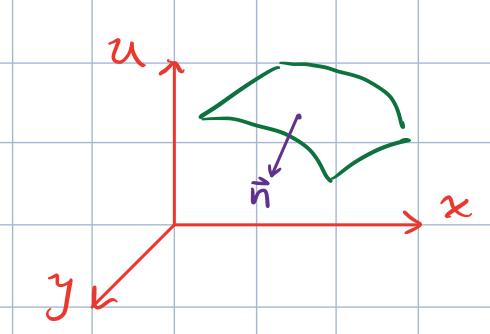
\includegraphics[scale=.75]{fig/fig2_method_characteristics.png}
	\caption{\captionStroke{Schematic integral surface with normal vector.}}
	\label{fig_normal_vector}
\end{figure}

We can rewrite the PDE as a dot product of the form
\begin{equation}
  \left\langle a(x, y), b(x, y), f(x, y, u) \right\rangle \cdot \mathbf{n} = 0.
\end{equation}

This implies that since the dot product is zero, the vector $\left\langle a(x,
y), b(x, y), f(x, y, u) \right\rangle$ must be normal to $\mathbf{n}$. Since we
stated that the vector $\mathbf{n}$ is normal to the surface $F(x, y, u) = 0$,
any vector $\mathbf{v}$ normal to $\mathbf{n}$ must lie in the tangential plane
to $F = 0$ at every point as depicted in
\begin{figure}[h!]
	\centering 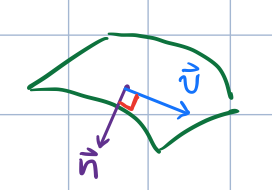
\includegraphics[scale=.75]{fig/fig3_method_characteristics.png}
	\caption{\captionStroke{Schematic integral surface with normal vector
  \mathbf{n} and tangential vector \matbf{v}.}}
	\label{fig_tangential_vector}
\end{figure}
